\documentclass[border=10pt]{standalone}

\usepackage{tikz}
\usepackage{tikzsymbols}
\usetikzlibrary{calc,patterns,shapes.geometric}

\def\centerarc[#1](#2)(#3:#4:#5){\draw[#1] ($(#2)+({#5*cos(#3)},{#5*sin(#3)})$) arc (#3:#4:#5);}

\begin{document}
	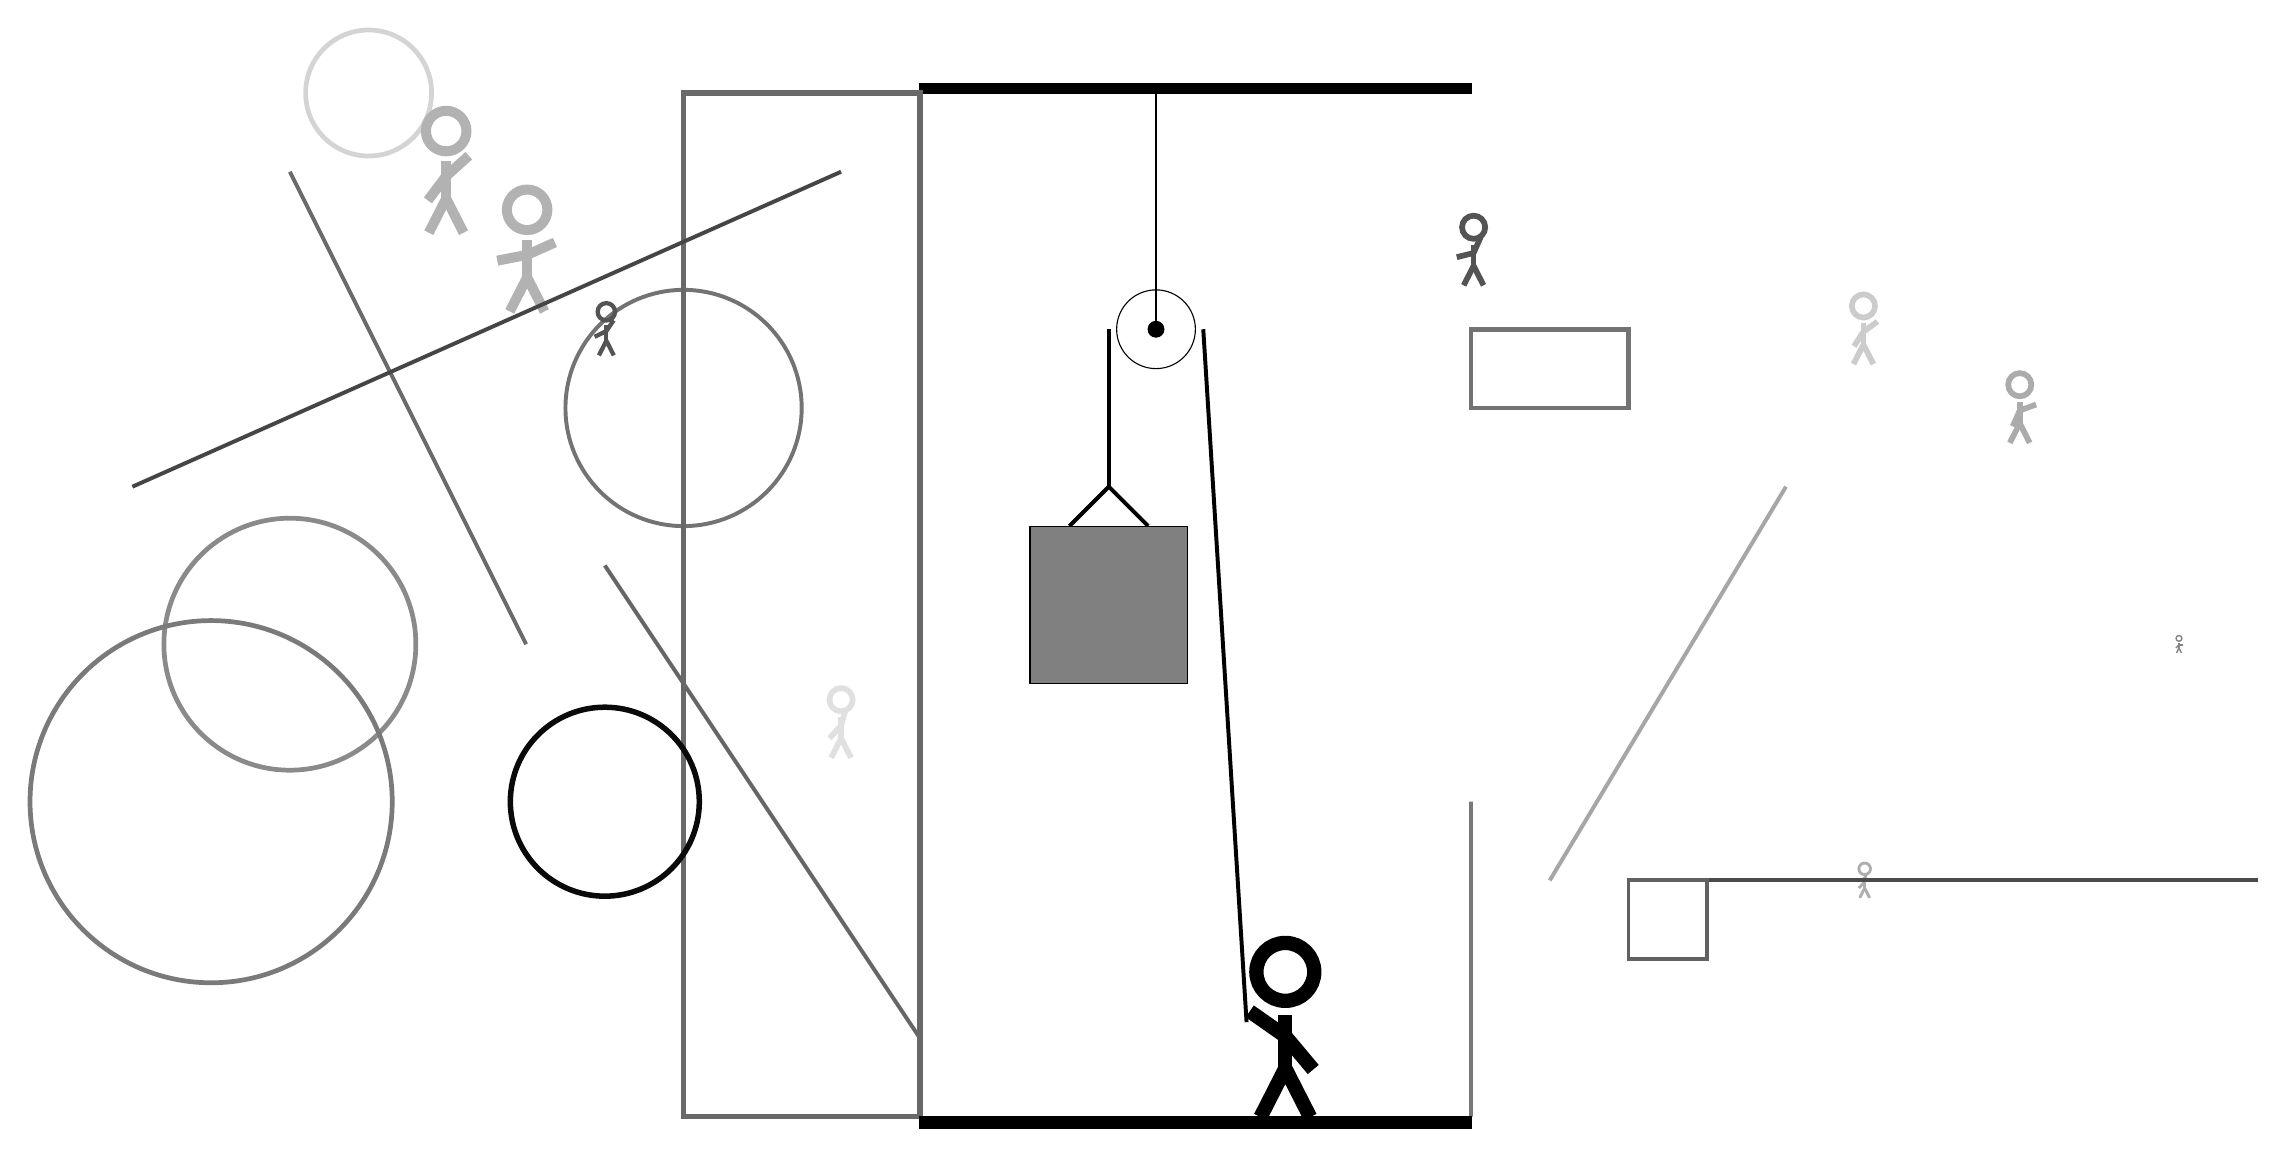
\begin{tikzpicture}
		%%%%% START %%%%%
		
		\draw[fill=black] (-2, 10) rectangle (5, 10.125);
		
		\draw (1, 7) circle (0.5);
		\draw[fill=black] (1, 7) circle (0.1);
		\draw (1, 10) -- (1, 7);
		
		\draw[line width=0.5mm] (-0.1, 4.5) -- (0.4, 5.0) -- (0.9, 4.5);
		\draw[fill=black!50] (-0.6, 4.5) rectangle (1.4, 2.5);
		
		\draw[line width=0.5mm] (0.4, 7) -- (0.4, 5.0);
		\centerarc[line width=0.5mm](1, 7)(0:180:0.6);
		\draw[line width=0.5mm](1.6, 7) -- (2.15, -1.8);
		
		\draw[line width=0.5mm, color=black!58](-7, 3) -- (-10, 9);
		
		\draw [line width=0.6mm, color=black!17](-9, 10) circle (0.8);
		\node[line width=0.2mm, color=black!30] at (-7, 8) {\Strichmaxerl[7][11][24]};
		\draw [line width=0.5mm, color=black!55](-5, 6) circle (1.5);
		\node[line width=0.3mm, color=black!30] at (-8, 9) {\Strichmaxerl[7][53][42]};
		\draw[line width=0.5mm, color=black!60](-6, 4) -- (-2, -2);
		
		\node[line width=0.3mm, color=black!48] at (14, 3) {\Strichmaxerl[1][46][0]};
		\draw[line width=0.5mm, color=black!35](9, 5) -- (6, 0);
		\draw[line width=0.6mm, color=black!55] (5, 7) rectangle (7, 6);
		
		\node[line width=0.4mm, color=black!67] at (-6, 7) {\Strichmaxerl[3][26][56]};
		\node[line width=0.2mm, color=black!12] at (-3, 2) {\Strichmaxerl[4][48][74]};
		\node[line width=0.5mm, color=black!32] at (10, 0) {\Strichmaxerl[2][48][82]};
		\node[line width=0.6mm, color=black!20] at (10, 7) {\Strichmaxerl[4][57][36]};
		
		\draw[line width=0.7mm, color=black!59] (-2, 10) rectangle (-5, -3);
		\draw[line width=0.5mm, color=black!71](8, 0) -- (15, 0);
		\node[line width=0.6mm, color=black!33] at (12, 6) {\Strichmaxerl[4][66][20]};
		\draw[line width=0.5mm, color=black!62] (7, 0) rectangle (8, -1);
		\draw[line width=0.5mm, color=black!73](-3, 9) -- (-12, 5);
		\draw [line width=0.7mm, color=black!96](-6, 1) circle (1.2);
		
		\node[line width=0.7mm, color=black!67] at (5, 8) {\Strichmaxerl[4][14][66]};
		\draw [line width=0.6mm, color=black!46](-10, 3) circle (1.6);
		
		\draw [line width=0.6mm, color=black!52](-11, 1) circle (2.3);
		\draw[line width=0.6mm, color=black!53] (5, -3) rectangle (5, 1);
		
		\node at (2.6, -1.9) {\Strichmaxerl[10][-35][-50]};
		
		\draw[fill=black] (-2, -3) rectangle (5, -3.15);
		
		%%%%% END %%%%%
	\end{tikzpicture}
\end{document}